% Define block styles
\tikzstyle{block} = [draw, rectangle, text centered, text width=10em, minimum height=0.5em, rounded corners=true]
\tikzstyle{arrowtext} = [text width=4em, text centered]
\tikzstyle{arrow} = [draw, -latex]

\definecolor{red1}{RGB}{160,0,0}
\definecolor{green1}{RGB}{0,160,0}
\definecolor{blue1}{RGB}{0,0,160}

	      
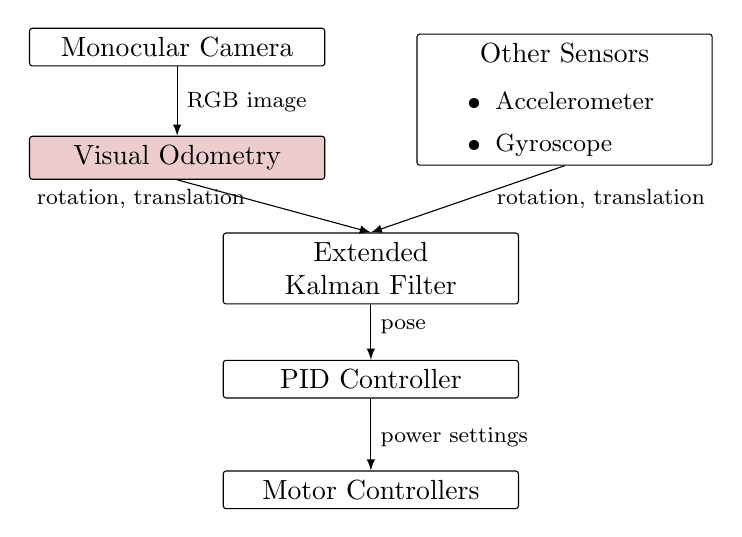
\begin{tikzpicture}[node distance=4em, auto]
	\node [block] (camera) {Monocular Camera};
	\node [block, below of=camera, fill=red1!20] (vo) {Visual Odometry};
	\node [block, below of=vo, xshift=7em] (kalman) {Extended Kalman Filter};
	\node [block, below of=kalman] (pid) {PID Controller};
	\node [block, below of=pid] (motor) {Motor Controllers};

	\node [block, right of=camera, node distance=14em, yshift=-1.9em] (sensors) {Other Sensors\\\small{\begin{itemize}\item Accelerometer \item Gyroscope\end{itemize}}};

	\draw [arrow] (camera.south) to (vo.north) node[right, yshift=1.2em] {\footnotesize RGB image};
	\draw [arrow] (vo.south) to (kalman.north) node[left, yshift=1.2em, xshift=-4.2em] {\footnotesize rotation, translation};
	\draw [arrow] (sensors.south) to (kalman.north) node[right, yshift=1.2em, xshift=4.2em] {\footnotesize rotation, translation};
	\draw [arrow] (kalman.south) to (pid.north) node[right, yshift=1.2em] {\footnotesize pose};
	\draw [arrow] (pid.south) to (motor.north) node[right, yshift=1.2em] {\footnotesize power settings};
\end{tikzpicture}
